\chapter{Principles of Image Partition Forests}
\label{chap:ipfs}

%---
\section{Chapter Overview}

This chapter introduces image partition forests (IPFs) as a data structure, and a core set of algorithms for working with them. As described here, IPFs are a data structure that can be applied to any type of image: they are not tied to the medical domain, although that is how they have been used in the project on which this thesis is based. Discussion of how to construct IPFs from medical images, and how to use them for identifying features therein, is deferred to Chapters~\ref{chap:segmentation} and \ref{chap:featureid}; in this chapter, we will take a more abstract view.

\vspace{\baselineskip}

\emph{Draft Version}

\def\acronym#1{\mbox{\textup{\textbf{#1}}}}

%---
\section{Overview}

The segmentation process I have implemented is based on the watershed/waterfall methods described in \cite{meijster98,marcotegui05}. At the highest possible level of abstraction, it can be seen to take an image (either 2D or 3D) as input, and produce an \emph{image partition forest} (IPF) for the image as output. Much of my research has involved developing algorithms which allow IPFs to be modified for the purposes of improving the segmentation or identifying important image features. This appendix describes IPFs and the algorithms I have developed for them. Their uses for segmentation and feature identification are described in \cite{gvccimi08,gvcispa09}.

% TODO: Figure here

%---
\section{Definition}

A formal definition for image partition forests can be built up as follows:

\begin{definition}
A set of $k$ objects $\{o_1,\ldots,o_k\}$ \textbf{partitions} object $o'$ iff $\bigcup_i o_i = o'$ and $\forall i,j \cdot i \ne j \Rightarrow o_i \cap o_j = \emptyset$. We write the relation as $\mathbf{P}(\{o_1,\ldots,o_k\},o')$.
\end{definition}

% TODO: Figure here

\begin{definition}
Given two object sets $O_f = \{o_{f1},\ldots,o_{fk(f)}\}$ and $O_c = \{o_{c1},\ldots,o_{ck(c)}\}$, and an object $o'$ partitioned by both $O_f$ and $O_c$, we say that $O_c$ is a \textbf{coarser partition} of $o'$ than $O_f$ (written $O_f \sqsubseteq O_c$) iff for every object $o_{ci} \in O_c$ there exists a subset $S_i \subseteq O_f$ such that $\mathbf{P}(S_i, o_{ci})$, and furthermore, $\forall i,j \in [1,k(c)] \cdot i \ne j \Rightarrow S_i \cap S_j = \emptyset$. (In other words, $O_f$ is a partition of $o'$ in which each individual object in $O_c$ has itself been partitioned.)
\end{definition}

% TODO: Figure here

\begin{definition}
Given a set of regions in an image $I$, $R_I = \{r_1,\ldots,r_k\}$, a function $w : R_I \times R_I \rightarrow \mathbb{R}^{+}$ is a \textbf{weight function} for $R_I$ iff $w(r_i,r_j) \ne \infty$ when, and only when, $r_i$ and $r_j$ are physically adjacent (share a common border) in $I$.
\end{definition}

% TODO: Figure here

\begin{definition}
A \textbf{weight function generator} is a function of type $\{\mbox{Region}\} \rightarrow (\{Region\} \times \{Region\} \rightarrow \mathbb{R}^{+})$. In particular, applying a weight function generator to a region set $R$ yields a weight function for $R$.
\end{definition}

\begin{definition}
The \textbf{region adjacency graph} $\mbox{RAG}_{\mbox{WFG}}(R_I)$ is the graph with nodes $r_i$ and edge weights given by the weight function $\mbox{WFG}(R_I)$.
\end{definition}

\begin{definition}
Let $T$ be a technique for generating image partition forests, and $\mbox{WFG}_T$ be its associated weight function generator. Given an image $I$, the \textbf{image partition forest} $\mbox{IPF}_{T}(I)$ is the sequence of $n_T$ pairs $[(P_{T0},\mbox{RAG}_{\mbox{WFG}_T}(P_{T0})),\ldots,(P_{T(n_T-1)},\mbox{RAG}_{\mbox{WFG}_T}(P_{T(n_T-1)}))]$, where $P_{Ti}$ is the $i^{th}$ partition produced by technique $T$ and satisfies $\mathbf{P}(P_{Ti},I)$, and $\forall i \in [0,n_T-1) \cdot P_{Ti} \sqsubseteq P_{T(i+1)}$. $P_{T0}$, the finest partition of $I$, is defined to be the pixel set of $I$ regardless of the generation technique employed.
\end{definition}

%---
\begin{figure}[p]
\begin{center}
	\subfigure[Source image]{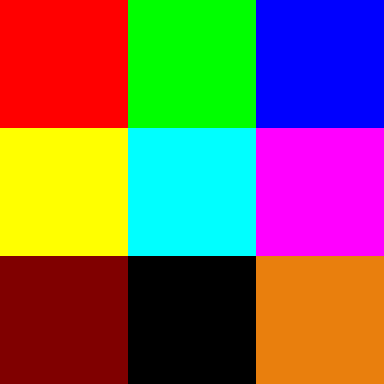
\includegraphics[height=6cm]{ipfs-example-image.png}}%
	\hspace{4mm}%
	\subfigure[Partition hierarchy: the red numbers indicate the number of pixels in each node, as an example property]{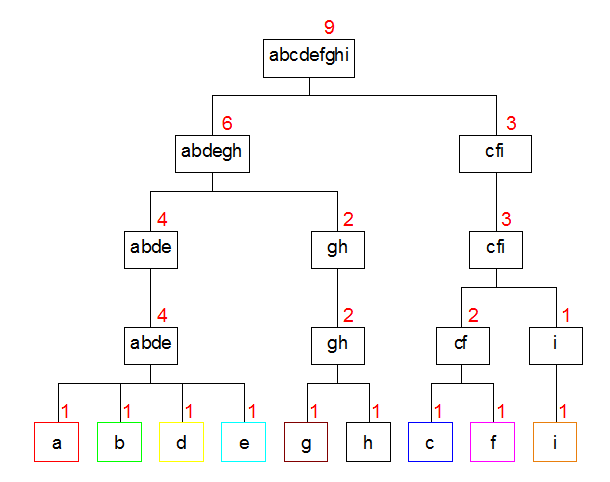
\includegraphics[height=6cm]{ipfs-example-hierarchy-coloured.png}}%
	\hspace{4mm}%
	\subfigure[RAG for layer 0 (the pixels of the image)]{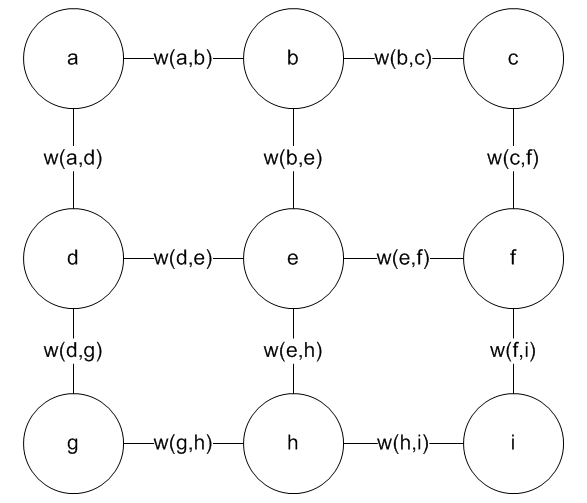
\includegraphics[height=6cm]{ipfs-example-rag0.png}}%
	\hspace{4mm}%
	\subfigure[RAG for layer 1]{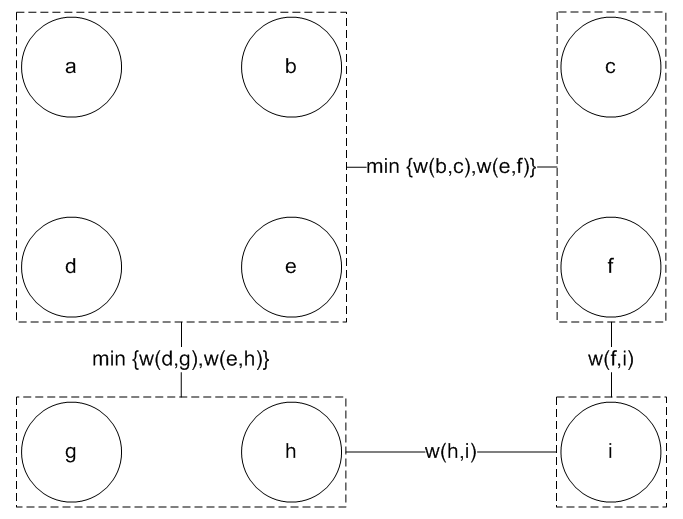
\includegraphics[height=6cm]{ipfs-example-rag1.png}}%
	\hspace{4mm}%
	\subfigure[RAG for layer 2]{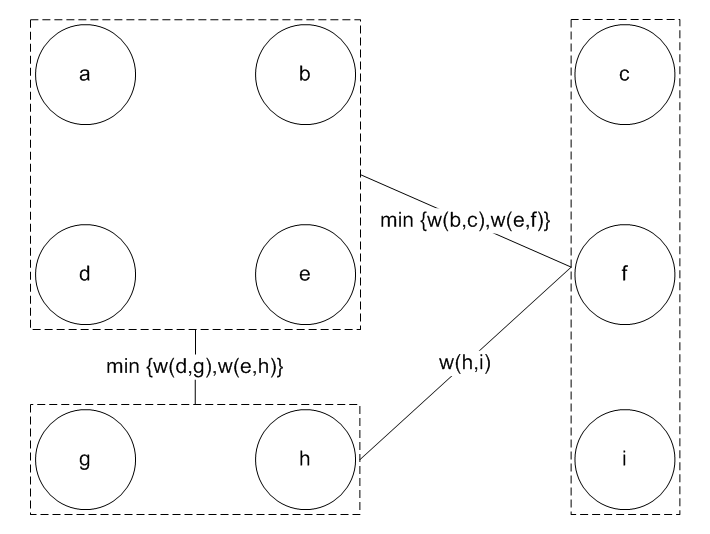
\includegraphics[height=6cm]{ipfs-example-rag2.png}}%
	\hspace{4mm}%
	\subfigure[RAG for layer 3]{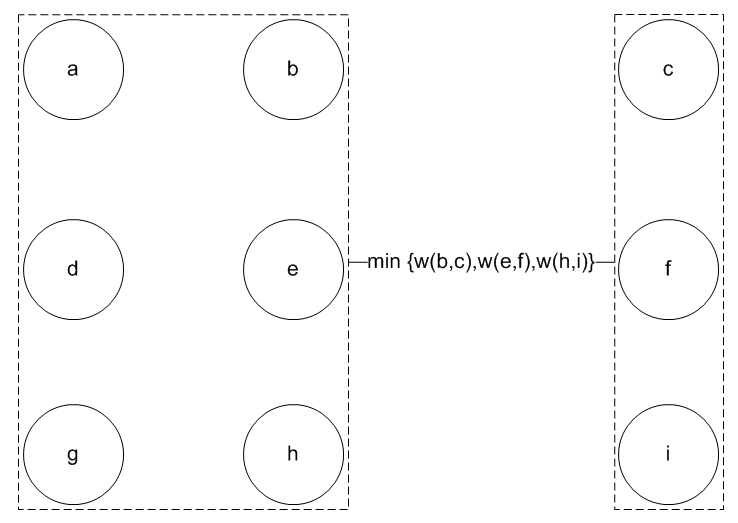
\includegraphics[height=6cm]{ipfs-example-rag3.png}}%
\end{center}
\caption{An example partition forest for a 3x3 2D image}
\label{fig:ipfs-example}
\end{figure}
%---

In my segmentation process, the technique $T$ is my particular watershed/waterfall approach, with $\mbox{WFG}_T$ being a weight function which generates weights corresponding to the `lowest pass point' between adjacent regions in the image (the lowest pass point between two adjacent regions is the lowest pixel value on the boundary between them). I also associate a set of properties (such as area, grey value mean, elongatedness, etc.) with each node in the forest for use in feature identification.

%---
\section{Algorithms}

\subsection{Fundamental Algorithms}

These are the core IPF algorithms on which all the more complicated algorithms rely. (A good way of thinking about it is that these are the ones which should definitely be member functions in an IPF class. The other algorithms could be implemented as free functions if desired.)

\subsubsection{Layer Creation}

New layers can be inserted anywhere in the hierarchy by cloning the layer above/below the insertion point (including its region adjacency graph and node properties). An IPF is guaranteed to have at least one layer (specifically, the lowest layer, corresponding to the pixel set of the image) at all times, so there will always be an existing layer to clone. The region adjacency graphs and node properties in existing layers are unaffected by the layer creation process. For an example, see Figure~\ref{fig:ipfs-layercreation}.

%---
\begin{figure}[H]
\begin{center}
	\subfigure[Before]{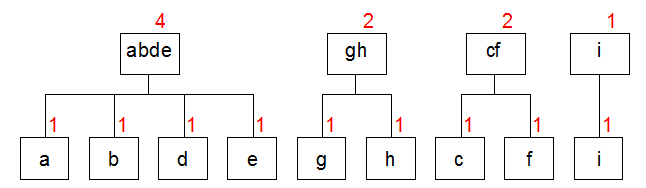
\includegraphics[width=8cm]{ipfs-layercreation-before.png}}%
	\hspace{4mm}%
	\subfigure[After cloning layer 0 to add a new layer between layers 0 and 1]{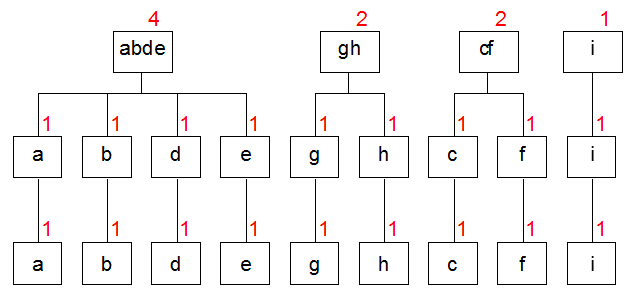
\includegraphics[width=8cm]{ipfs-layercreation-after.png}}%
\end{center}
\caption{Layer Creation Example}
\label{fig:ipfs-layercreation}
\end{figure}
%---

\subsubsection{Layer Deletion}

Any IPF layer other than the lowest layer can be deleted from the hierarchy. This process involves not only removing the layer, but modifying the parent/child pointers in any layers either side of the one being removed. The region adjacency graphs and node properties in other layers are unaffected by the layer deletion process. For an example, see Figure~\ref{fig:ipfs-layerdeletion}.

%---
\begin{figure}[H]
\begin{center}
	\subfigure[Before]{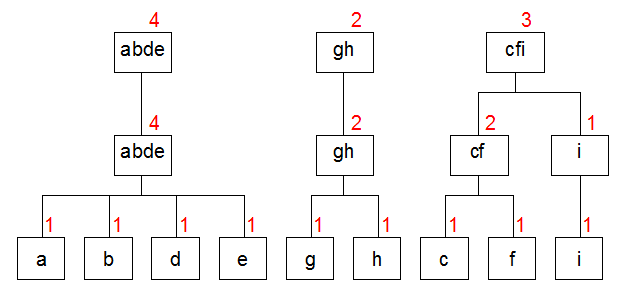
\includegraphics[width=8cm]{ipfs-layerdeletion-before.png}}%
	\hspace{4mm}%
	\subfigure[After deleting layer 1]{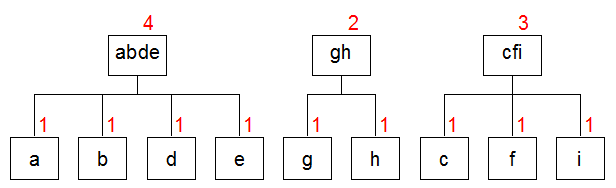
\includegraphics[width=8cm]{ipfs-layerdeletion-after.png}}%
\end{center}
\caption{Layer Deletion Example}
\label{fig:ipfs-layerdeletion}
\end{figure}
%---

\subsubsection{Region Splitting}

Regions in any layer other than the lowest (containing the image pixels) can be split into several contiguous components (each specified as a set of nodes which are children of the node to be split). This involves the following steps:

\begin{enumerate}

\item Check that the node to be split is not in the bottom layer of the hierarchy.
\item Check that each component is contiguous (for each component of size greater than 1, flood out from the first node -- only recursing to adjacent nodes also in the component -- and make sure they all get reached).
\item Remove the links between the initial parent (the node being split) and its children.
\item Create new nodes as necessary for all but one of the components (we reuse the initial parent for one of them) and link them to the initial grandparent (the parent of the node being split), if any.
\item Link the child nodes to their new parents and calculate the properties of the component parents from them.
\item Locally recalculate the region adjacency graph for the layer in which the node was split (disconnect the initial parent -- since some of the edges for it will no longer be valid -- and then recalculate the edges for all component parents using the region adjacency graph for the layer below).

\end{enumerate}

\noindent An example of this process is shown in Figure~\ref{fig:ipfs-regionsplitting}.

%---
\begin{figure}[ht]
\begin{center}
	\subfigure[Initial hierarchy]{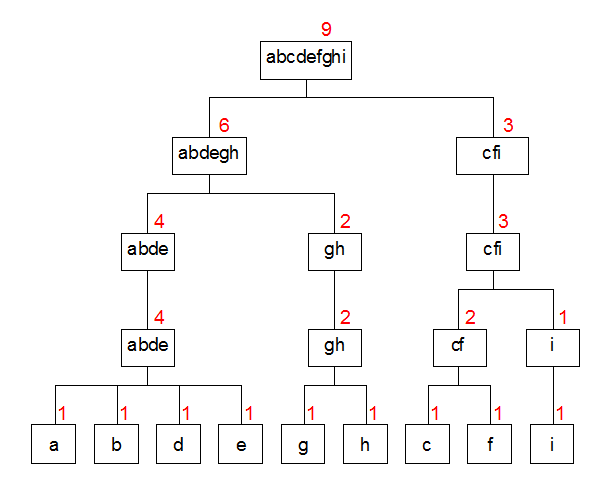
\includegraphics[height=6cm]{ipfs-example-hierarchy.png}}%
	\hspace{4mm}%
	\subfigure[Initial layer 1 RAG]{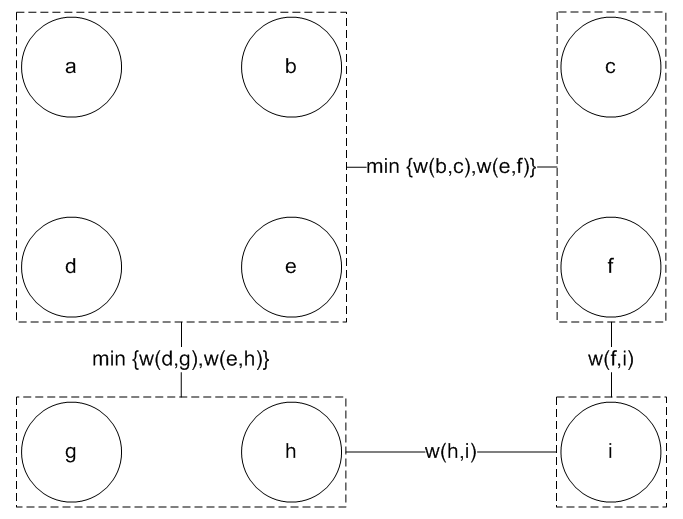
\includegraphics[height=6cm]{ipfs-example-rag1.png}}%
	\hspace{4mm}%
	\subfigure[Hierarchy after step 3]{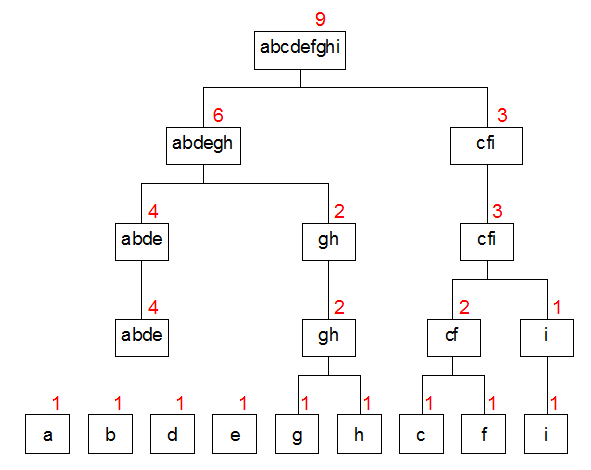
\includegraphics[height=6cm]{ipfs-regionsplitting-step3.png}}%
	\hspace{4mm}%
	\subfigure[Hierarchy after step 4]{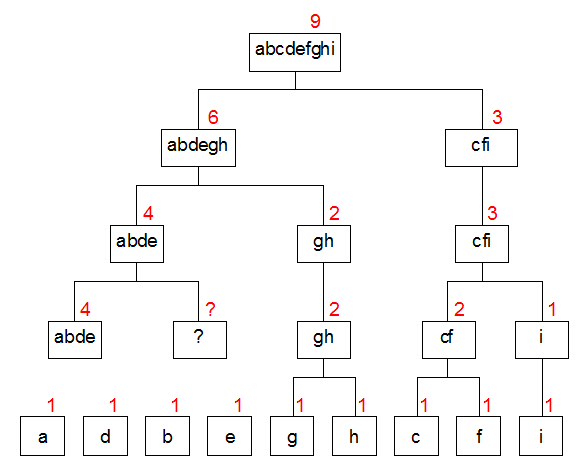
\includegraphics[height=6cm]{ipfs-regionsplitting-step4.png}}%
	\hspace{4mm}%
	\subfigure[Hierarchy after step 5]{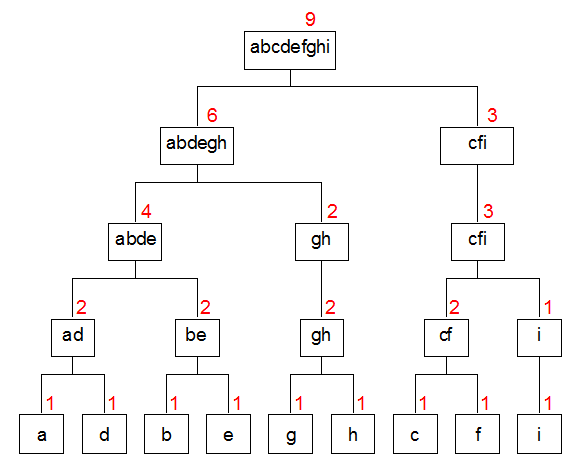
\includegraphics[height=6cm]{ipfs-regionsplitting-step5.png}}%
	\hspace{4mm}%
	\subfigure[Layer 1 RAG after step 6]{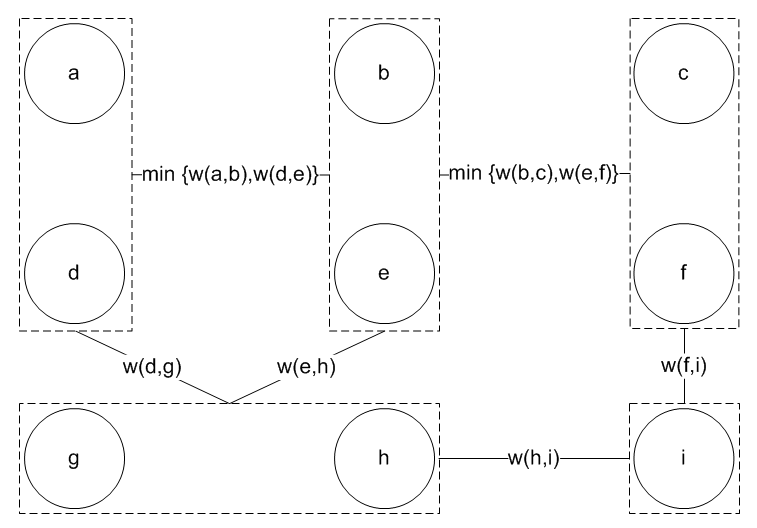
\includegraphics[height=6cm]{ipfs-regionsplitting-step6.png}}%
\end{center}
\caption{Region Splitting Example: Split (1,abde) into \{(0,a), (0,d)\} and \{(0,b), (0,e)\}}
\label{fig:ipfs-regionsplitting}
\end{figure}
%---

\subsubsection{Sibling Region Merging}

Sibling regions (i.e. those with the same parent) in any region other than the lowest (containing the image pixels) can be merged if their union would be a contiguous region. This involves the following steps:

\begin{enumerate}

\item Check that the nodes to be merged are not in the bottom layer.
\item Check that the merge result would be a contiguous region (this can be done using the method described in step 2 of \emph{Region Splitting}, above).
\item Pick one of the nodes to be merged to be reused as the new combined node, and set the parent links of the other nodes' children to point to it.
\item Remove the links between the (now redundant) other nodes and their parent and delete them.
\item Recalculate the properties of the combined node.
\item Merge the nodes in the region adjacency graph for their layer.

\end{enumerate}

\noindent An example of this process is shown in Figure~\ref{fig:ipfs-siblingmerging}.

%---
\begin{figure}[ht]
\begin{center}
	\subfigure[Initial hierarchy]{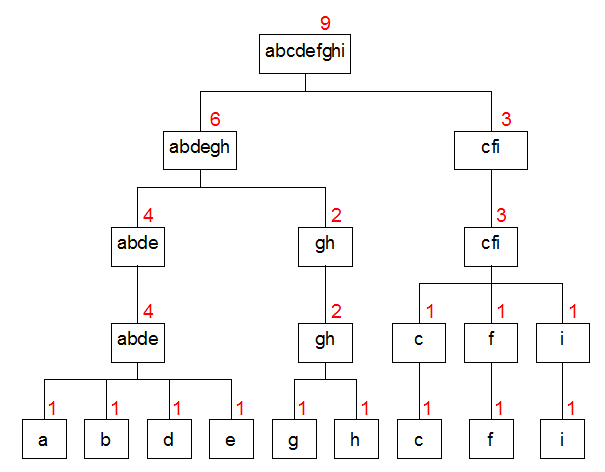
\includegraphics[height=6cm]{ipfs-siblingmerging-initialhierarchy.png}}%
	\hspace{4mm}%
	\subfigure[Initial layer 1 RAG]{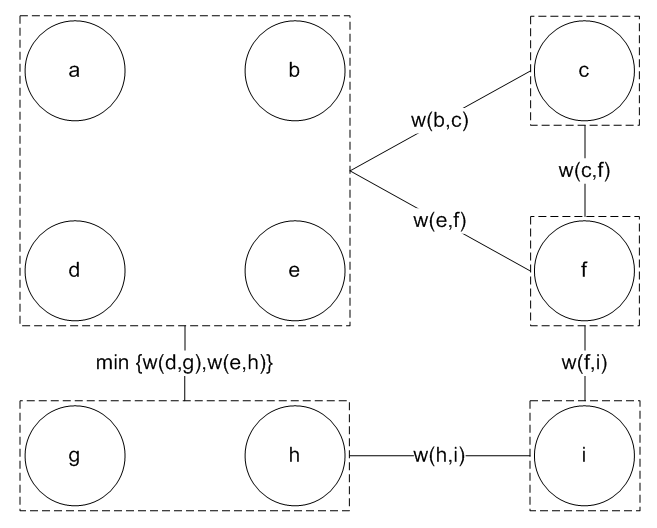
\includegraphics[height=6cm]{ipfs-siblingmerging-initialrag1.png}}%
	\hspace{4mm}%
	\subfigure[Hierarchy after step 3]{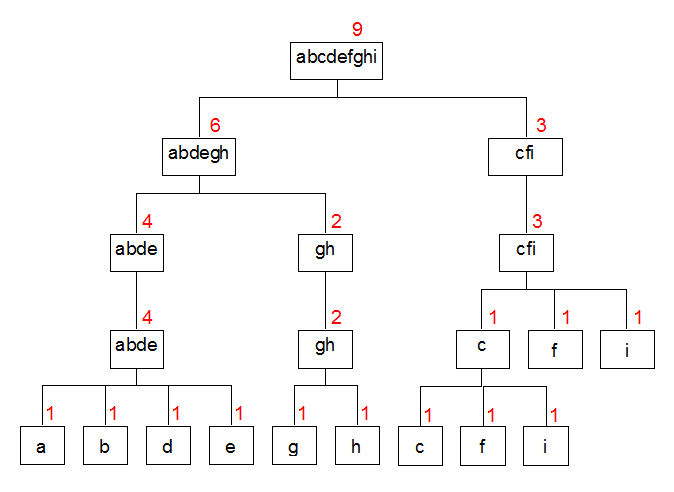
\includegraphics[height=6cm]{ipfs-siblingmerging-step3.png}}%
	\hspace{4mm}%
	\subfigure[Hierarchy after step 4]{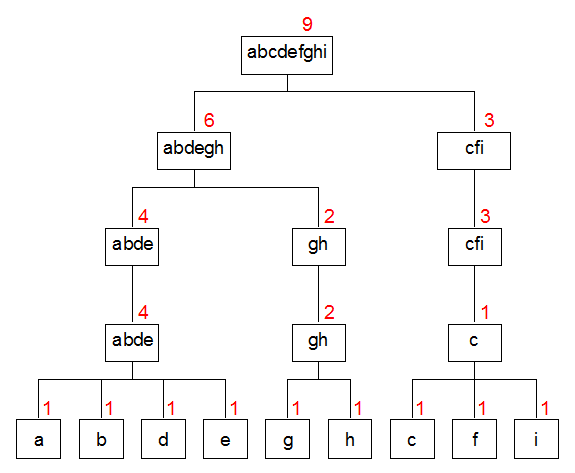
\includegraphics[height=6cm]{ipfs-siblingmerging-step4.png}}%
	\hspace{4mm}%
	\subfigure[Hierarchy after step 5]{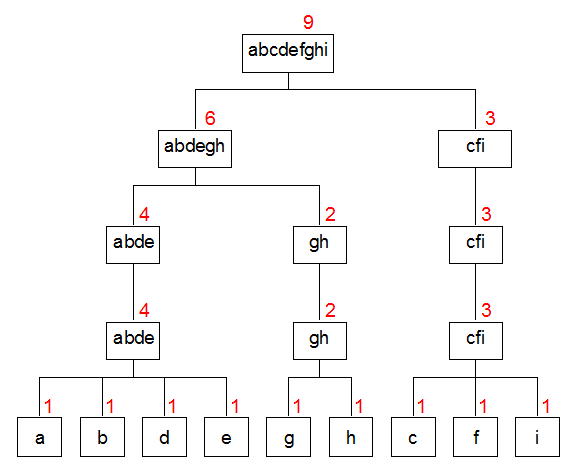
\includegraphics[height=6cm]{ipfs-siblingmerging-step5.png}}%
	\hspace{4mm}%
	\subfigure[Layer 1 RAG after step 6]{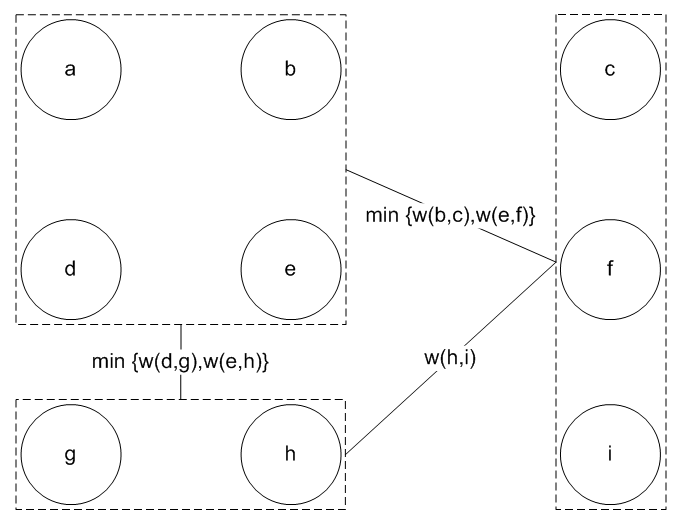
\includegraphics[height=6cm]{ipfs-siblingmerging-step6.png}}%
\end{center}
\caption{Sibling Region Merging Example: Merge (1,c), (1,f) and (1,i)}
\label{fig:ipfs-siblingmerging}
\end{figure}
%---

\subsection{Zipping Algorithms}

The next layer of algorithms up are zipping algorithms. These are effectively splitting/merging algorithms for branches rather than individual regions, and are fundamental subroutines of the applied algorithms described subsequently.

\subsubsection{Unzipping}

A region in any layer of the hierarchy (including the lowest layer) can be unzipped to a specified higher layer (or the top of the hierarchy). This essentially `separates out' the branch from the higher layer down to the specified region (it's effectively a multi-layer split). It involves the following steps:

\begin{enumerate}

\item Let $\mathit{cur}$ be the node to be unzipped.
\item While the layer of $\mathit{cur}$ is less than the specified higher layer and $\mathit{cur}$ has a parent:

\begin{enumerate}
\item Let $p = \mbox{parent}(\mathit{cur})$ and $S = \mbox{children}(p) \; \backslash \; \mathit{cur}$.
\item Calculate $\mathit{CCS}$ as the connected components of $S$.
\item Split $p$ into $\mathit{CCS} \cup \{\mathit{cur}\}$.
\item Set $\mathit{cur} = \mbox{parent}(\mathit{cur})$.
\end{enumerate}

\end{enumerate}

\noindent See Figures~\ref{fig:ipfs-unzipping1} and \ref{fig:ipfs-unzipping2} for examples (note that the RAGs are not shown for brevity).

%---
\begin{figure}[p]
\begin{center}
	\subfigure[Initial hierarchy]{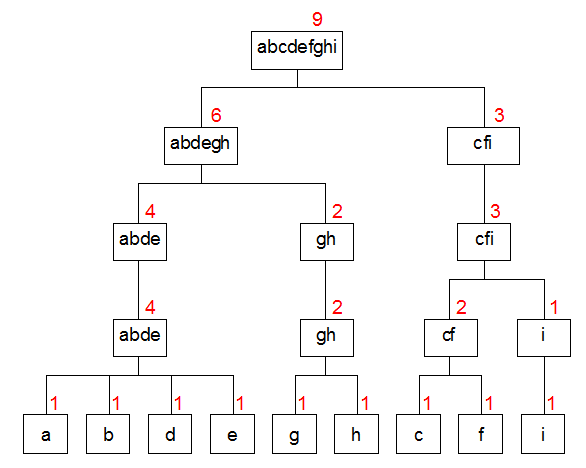
\includegraphics[height=6cm]{ipfs-unzipping1-initialhierarchy.png}}%
	\hspace{4mm}%
	\subfigure[After layer 1 split]{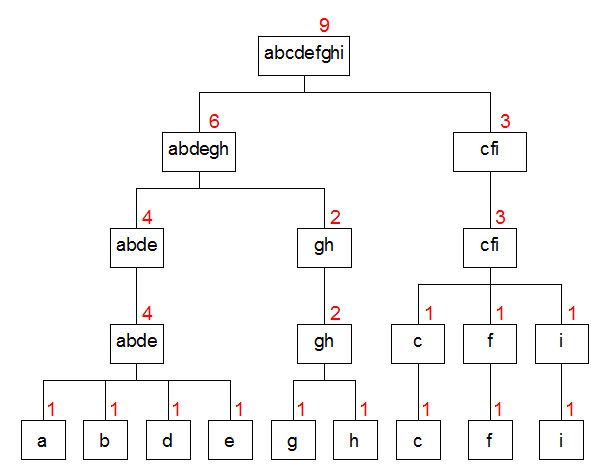
\includegraphics[height=6cm]{ipfs-unzipping1-split1.png}}%
	\hspace{4mm}%
	\subfigure[After layer 2 split]{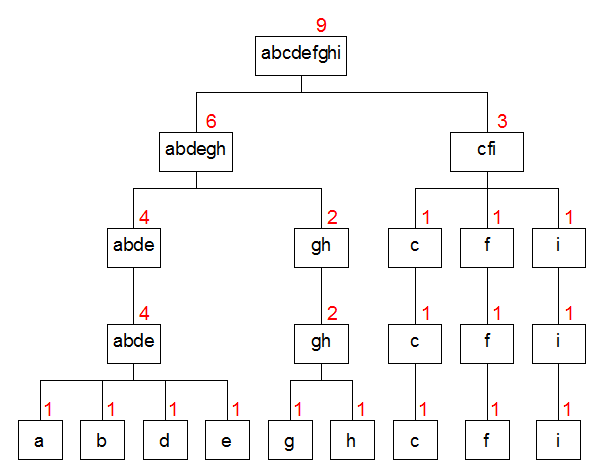
\includegraphics[height=6cm]{ipfs-unzipping1-split2.png}}%
	\hspace{4mm}%
	\subfigure[After layer 3 split]{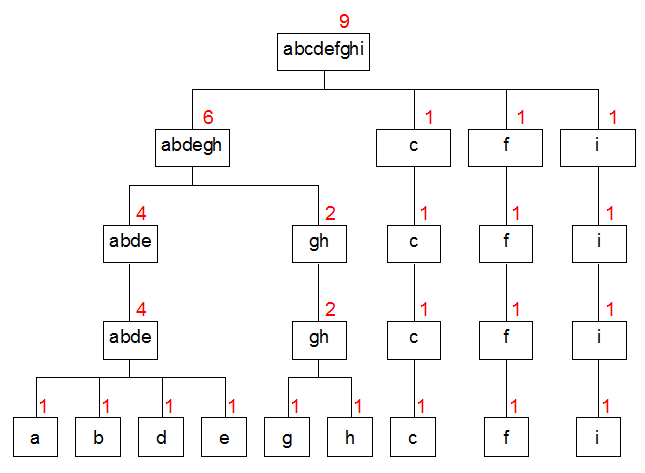
\includegraphics[height=6cm]{ipfs-unzipping1-split3.png}}%
\end{center}
\caption{Unzipping Example \#1: Unzip (0,f) to layer 3}
\label{fig:ipfs-unzipping1}
\end{figure}
%---

%---
\begin{figure}[p]
\begin{center}
	\subfigure[Initial hierarchy]{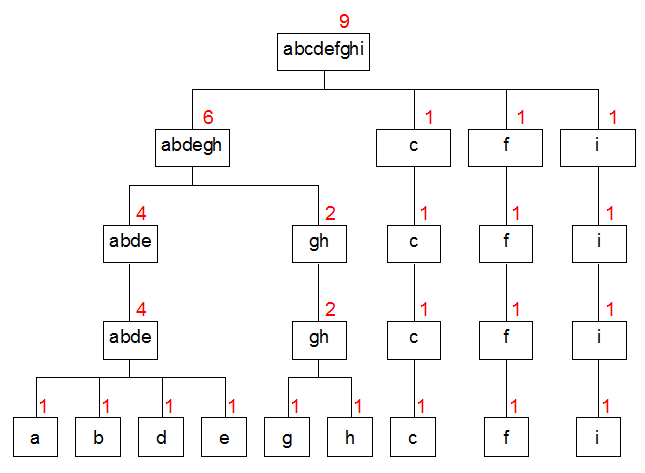
\includegraphics[height=6cm]{ipfs-unzipping1-split3.png}}%
	\hspace{4mm}%
	\subfigure[After layer 1 split]{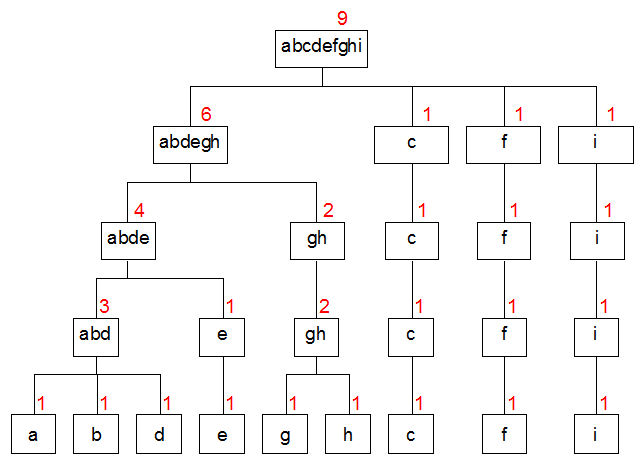
\includegraphics[height=6cm]{ipfs-unzipping2-split1.png}}%
	\hspace{4mm}%
	\subfigure[After layer 2 split]{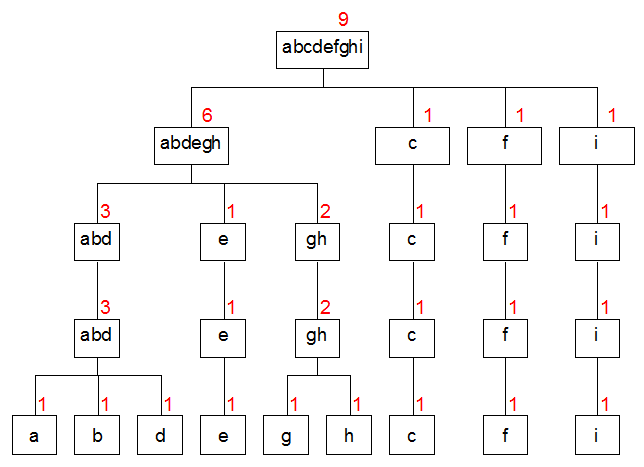
\includegraphics[height=6cm]{ipfs-unzipping2-split2.png}}%
	\hspace{4mm}%
	\subfigure[After layer 3 split]{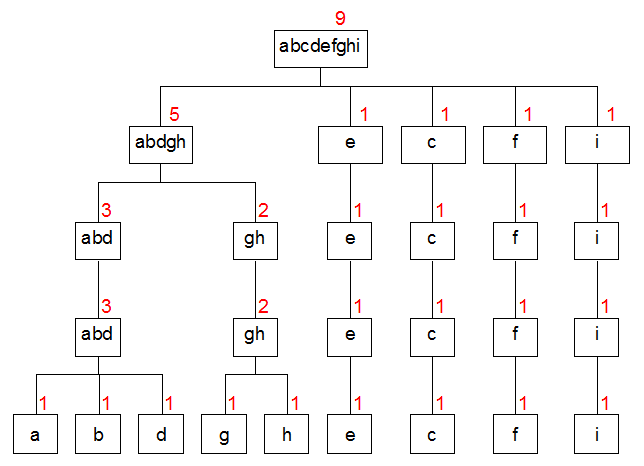
\includegraphics[height=6cm]{ipfs-unzipping2-split3.png}}%
\end{center}
\caption{Unzipping Example \#2: Unzip (0,e) to layer 3}
\label{fig:ipfs-unzipping2}
\end{figure}
%---

\subsubsection{Zipping}

\begin{definition}
An \textbf{$h$---$\ell$ chain} of nodes is a sequence of nodes $[n_0,\ldots,n_{h-\ell}]$, where $n_i$ is in layer $h-i$ and $\forall i > 0 \cdot \mbox{parent}(n_i) = n_{i-1}$.
\end{definition}

For any given $h$ and $\ell$ (provided $\ell > 0$, since pixels cannot be merged), it is possible to zip together multiple $h$---$\ell$ chains, a process which is effectively a multi-layer merge. For this to work, the highest nodes in each of the chains must share a common parent (i.e.~they must be siblings) and the union of the lowest nodes in the chains must be a contiguous region. The process is then straightforward. Given $k$ chains $[n_{00},\ldots,n_{0(h-\ell)}]$, $\ldots$, $[n_{k0},\ldots,n_{k(h-\ell)}]$, the algorithm is thus as follows:

\begin{enumerate}

\item Check that $n_{00}, \ldots, n_{k0}$ have a common parent (or are in the highest layer of the hierarchy).

\item Check that the union of the lowest nodes (i.e.~$n_{0(h-\ell)}, \ldots, n_{k(h-\ell)}$) will be contiguous.

\item For $i$ = $0$ to $h - \ell$:

\begin{enumerate}
\item Perform a sibling region merge on $n_{0i}, \ldots, n_{ki}$.
\end{enumerate}

\end{enumerate}

\noindent Notes:

\begin{itemize}

\item There is no need to check that other corresponding nodes in the chains are siblings before attempting a sibling merge: merging their parents in the previous iteration of the loop will automatically guarantee that they share the same parent.

\item The zipping process can (as one might expect) be used to reverse the unzipping process described in the previous subsection, provided the unzipping is implemented to return the relevant chains of nodes. (This is useful when it comes to implementing undoable operations: the alternative of storing a copy of the old hierarchy for later restoration is obviously far more costly.)

\end{itemize}

\noindent See Figure~\ref{fig:ipfs-zipping} for an example of the process.

%---
\begin{figure}[p]
\begin{center}
	\subfigure[Initial hierarchy]{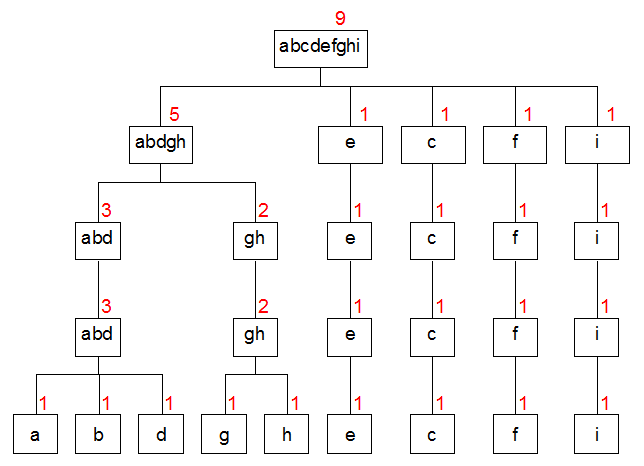
\includegraphics[height=6cm]{ipfs-unzipping2-split3.png}}%
	\hspace{4mm}%
	\subfigure[After layer 3 merge]{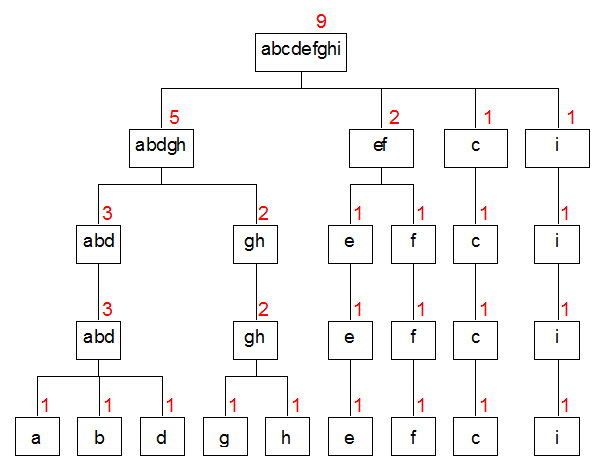
\includegraphics[height=6cm]{ipfs-zipping-merge1.png}}%
	\hspace{4mm}%
	\subfigure[After layer 2 merge]{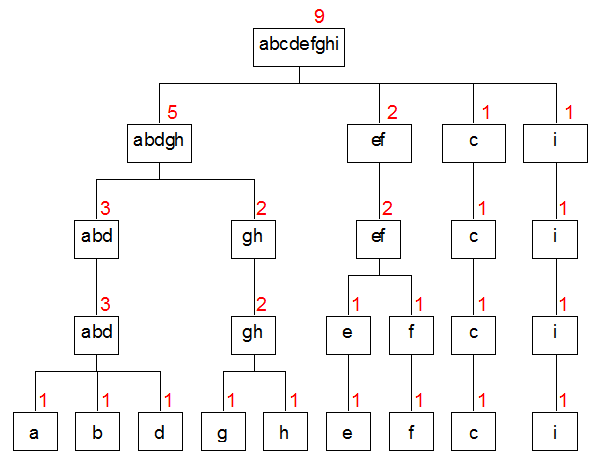
\includegraphics[height=6cm]{ipfs-zipping-merge2.png}}%
	\hspace{4mm}%
	\subfigure[After layer 1 merge]{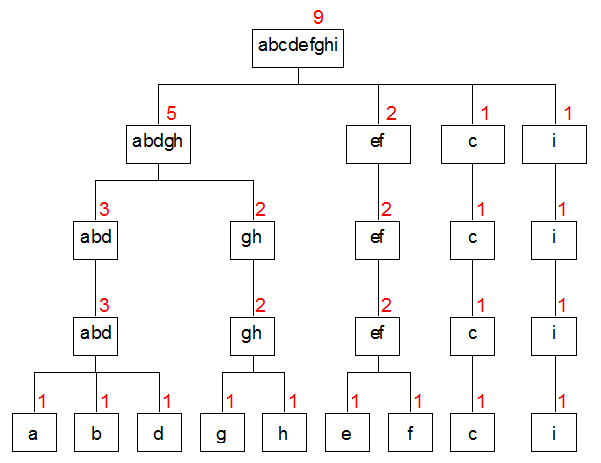
\includegraphics[height=6cm]{ipfs-zipping-merge3.png}}%
\end{center}
\caption{Zipping Example: Zipping [(3,e),(2,e),(1,e)] to [(3,f),(2,f),(1,f)]}
\label{fig:ipfs-zipping}
\end{figure}
%---

\subsection{Applied Algorithms}

%The highest layer of algorithms are the applied algorithms. These are built on top of the zipping algorithms described previously.

\subsubsection{Feature Identification}

Some medical imaging applications (for example visualization of the body in 3D using e.g.~the multiple material marching cubes algorithm \cite{wu03}) require a labelled volume as input. It is thus important to be able to mark nodes in the partition forest with a given label, e.g.~`KIDNEY' or `LIVER'. To do this, it is unfortunately not sufficient to simply set a label property in the selected node. Assigning a label to a node implicitly assigns that label to all its descendants (since it contains them). It also affects the labels of its ancestors: for example, if a node is labelled as `KIDNEY', then at least part of its parent (which contains it) is also `KIDNEY'. Since we ultimately want regions to have semantic meaning, it makes little sense to start having complex labels which are part one thing and part another. We therefore take the alternative approach of unzipping the tree instead. The algorithm is as follows:

\begin{enumerate}

\item Unzip the region to be marked to the top of the hierarchy.
\item Assign the given label to the entire tree in which the unzipped region resides.

\end{enumerate}

An example of the process is shown in Figure~\ref{fig:ipfs-featureid}. Note that whilst the second step of the algorithm might seem like a costly process (since it seems like you have to traverse the entire tree), it would suffice in practice to simply mark the top node and specify that the feature ID for each node not in the top layer of the hierarchy is given by that of its highest-layer ancestor.

%---
\begin{figure}[p]
\begin{center}
	\subfigure[Initial hierarchy]{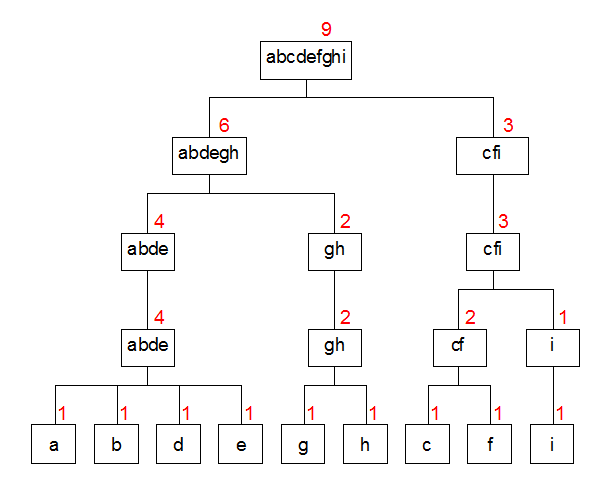
\includegraphics[height=6cm]{ipfs-example-hierarchy.png}}%
	\hspace{4mm}%
	\subfigure[After step 1]{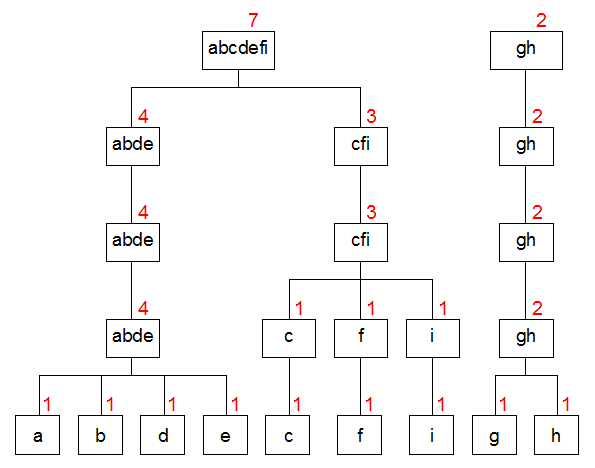
\includegraphics[height=6cm]{ipfs-featureid-step1.png}}%
	\hspace{4mm}%
	\subfigure[After step 2]{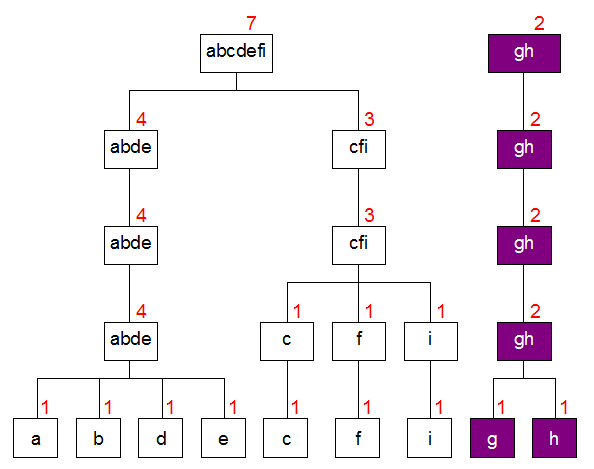
\includegraphics[height=6cm]{ipfs-featureid-step2.png}}%
\end{center}
\caption{Feature Identification Example: Identifying (1,gh) as `purple'}
\label{fig:ipfs-featureid}
\end{figure}
%---

\subsubsection{Arbitrary Region Merging}

It is not just siblings in the same layer which can be merged: arbitrary regions in the same layer can be as well. This can be useful when (say) several pieces of the same organ have ended up belonging to different parents in the layer above. The process is more complicated than before, however:

\begin{enumerate}

\item Check that the nodes to be merged are not in the bottom layer.

\item Calculate $\mathit{CCS}$ as the connected components of the regions to be merged.

\item For each $\mathit{cc} \in \mathit{CCS}$ such that $|\mathit{cc}| > 1$:

\begin{enumerate}
\item Find the common ancestor, $a$, of the regions in $\mathit{cc}$ (note that $a$ is allowed to be the top of the hierarchy if the regions have no common ancestor).
\item Unzip each region in $\mathit{cc}$ in turn to the layer below that of $a$.
\item Zip the strands thus created for each region in $\mathit{cc}$ together to merge the regions.
\end{enumerate}

\end{enumerate}

\noindent An example of this process in action is shown in Figure~\ref{fig:ipfs-arbitrarymerge}.

%---
\begin{figure}[p]
\begin{center}
	\subfigure[Initial hierarchy]{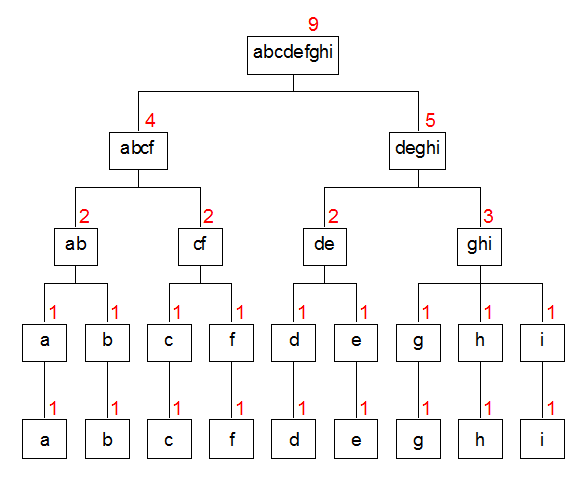
\includegraphics[height=6cm]{ipfs-arbitrarymerge1.png}}%
	\hspace{4mm}%
	\subfigure[After step 3b for first component]{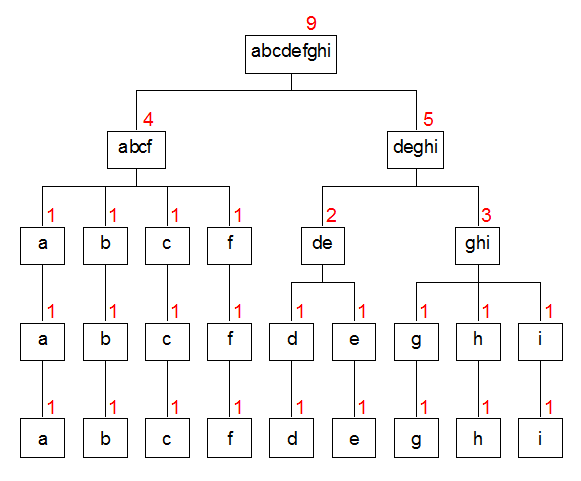
\includegraphics[height=6cm]{ipfs-arbitrarymerge2.png}}%
	\hspace{4mm}%
	\subfigure[After step 3c for first component]{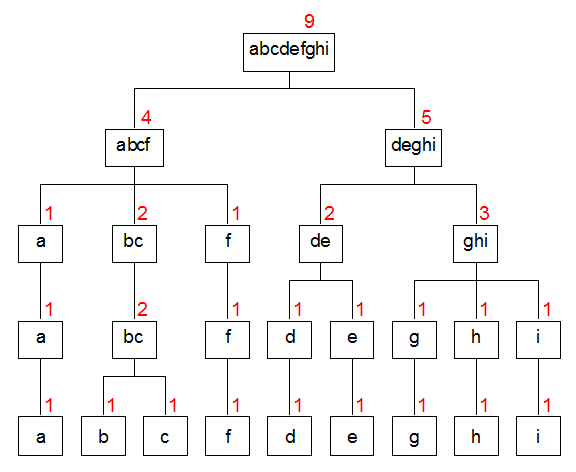
\includegraphics[height=6cm]{ipfs-arbitrarymerge3.png}}%
	\hspace{4mm}%
	\subfigure[After step 3b for second component]{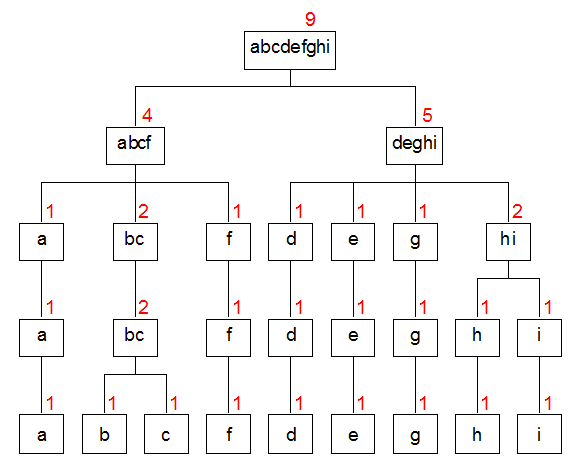
\includegraphics[height=6cm]{ipfs-arbitrarymerge4.png}}%
	\hspace{4mm}%
	\subfigure[After step 3c for second component (result)]{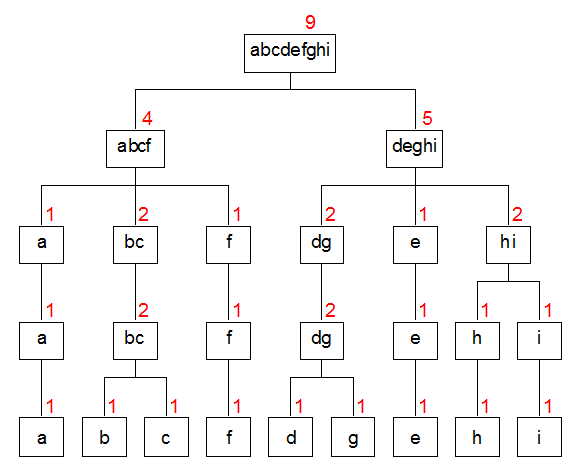
\includegraphics[height=6cm]{ipfs-arbitrarymerge5.png}}%
\end{center}
\caption{Arbitrary Region Merging Example: Merging (1,b), (1,c), (1,d) and (1,g)}
\label{fig:ipfs-arbitrarymerge}
\end{figure}
%---

\subsubsection{Parent Switching}

A node in any layer of the hierarchy except the highest can be moved from being the child of its parent node to being the child of another node in the layer above, provided that it is adjacent to at least one child of its new parent. The process is as follows:

\begin{enumerate}
\item Check that the node ($n$) is adjacent to at least one child of its proposed new parent using the region adjacency graph for the node's layer.
\item Find the common ancestor, $a$ of the old and new parents (note that $a$ is allowed to be the top of the hierarchy if the nodes have no common ancestor).
\item Unzip $n$ to the layer below that of $a$.
\item Zip the strand thus created to the strand leading from $a$ down to the new parent.
\end{enumerate}

\noindent See Figure~\ref{fig:ipfs-parentswitching} for an example.

%---
\begin{figure}[p]
\begin{center}
	\subfigure[Initial hierarchy]{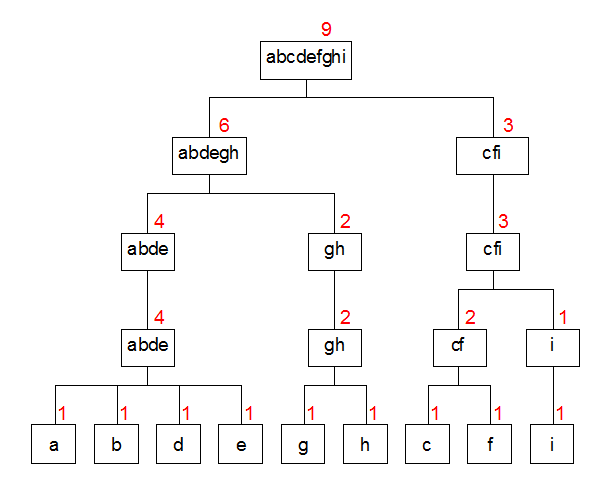
\includegraphics[height=6cm]{ipfs-example-hierarchy.png}}%
	\hspace{4mm}%
	\subfigure[After step 3]{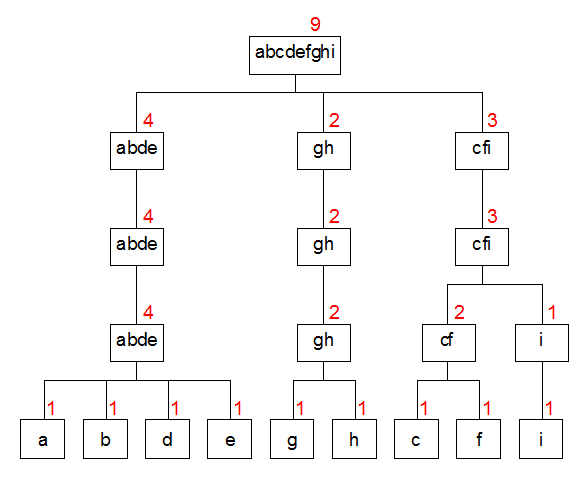
\includegraphics[height=6cm]{ipfs-parentswitching1.png}}%
	\hspace{4mm}%
	\subfigure[After step 4]{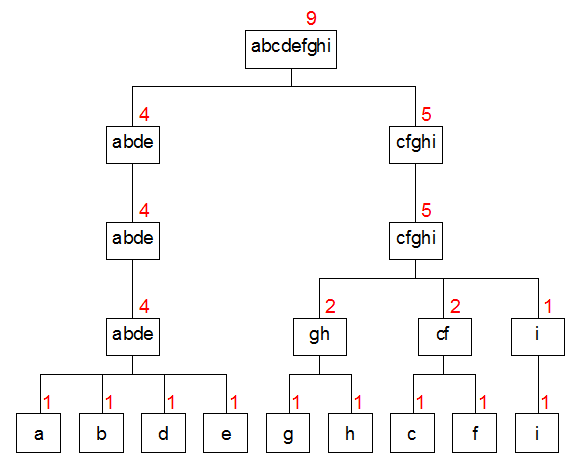
\includegraphics[height=6cm]{ipfs-parentswitching2.png}}%
\end{center}
\caption{Parent Switching Example: Reparent (1,gh) to (2,cfi)}
\label{fig:ipfs-parentswitching}
\end{figure}
%---

\subsection{Selection Algorithms}

The ability to select nodes from multiple layers in an IPF is important because it enables more sophisticated editing techniques for the end-user. It is evidently straightforward to allow the selection of individual IPF nodes: we simply come up with a node identification scheme -- e.g.~the $(\mathit{layer},\mathit{\{letters\}})$ system used in this report -- and store an identifier to refer to the currently selected node. In a more practical scheme, however, it would be possible to (for example) select a node in one layer and view it in terms of its sub-regions at the next layer down: this would allow the user to select a large region and then remove any of its sub-regions which should not actually have been selected. This is the motivation behind the idea of multi-layer node selection, in which we view the selection of an IPF node not as the selection of just a single node, but of the entire subtree beneath it. In other words, if we select a node, we implicitly select all of its descendants.

Implementing this could be done na\"ively by storing all the nodes selected in every level of the tree, but that would be deeply inefficient. Instead, as described in \cite{gvcispa09}, we define a minimal node representation ($\acronym{MNR}$) for the selection and use that. We note that any selection of regions in an image is really just a selection of some (or all) of the image pixels. Letting $\mathbf{PS}(I)$ be the pixel set of image $I$, and the current selection be a set of pixels $S \subseteq \mathbf{PS}(I)$, we define $\acronym{MNR}(S)$ to be the smallest set of nodes that represents $S$. For example, in Figure~\ref{fig:ipfs-mnr}, consider the selection $S$ of the pixels $(0,d)$, $(0,g)$ and $(0,h)$: in this case $\acronym{MNR}(S) = \{(0,d),(1,\mathit{gh})\}$. If we then removed the pixel $(0,h)$ from the selection, $\acronym{MNR}(S)$ would become $\{(0,d),(0,g)\}$.

%---
\stufigex{height=6cm}{ipfs-mnr.png}{An example showing the minimal node representation (in grey) for the selection of the pixels $(0,d)$, $(0,g)$ and $(0,h)$}{fig:ipfs-mnr}{ht}
%---

Having defined such a minimal node representation, there are three key operations we need to support on it: adding nodes, removing them, and viewing the selection at a particular layer in the hierarchy. Adding a node ensures that all the pixels in the region represented by the node are `in the selection'. Removing a node ensures that no pixel in the region remains in the selection. Viewing the selection at a given layer allows us to select a node in one layer of the hierarchy and then view it as its constituent sub-regions in the layers below. From an end-user perspective, it is helpful if changes to the selection are undoable: this can easily be accomplished by recording which node identifiers are added and removed from $\acronym{MNR}(S)$ by each operation.

\subsubsection{Add to Selection}

There are four cases to deal with when adding a node to the selection:

\begin{enumerate}

\item The node is already in $\acronym{MNR}(S) \Rightarrow $ do nothing.

\item An ancestor of the node is already in $\acronym{MNR}(S) \Rightarrow $ do nothing.

\item One or more descendants of the node are already in $\acronym{MNR}(S)$: we remove them and add this node instead, since it contains all its descendants.

\item Otherwise: simply add the node to $\acronym{MNR}(S)$ directly.

\end{enumerate}

If we added a node identifier (either of the latter two cases), we need to \emph{consolidate} the selection as a final step: this involves replacing any node whose children are all selected with the node itself in \acronym{MNR}(S). We only need to consider nodes which might have been affected by the new node addition when performing this process: thus, it suffices to recursively consolidate nodes from the parent of the added node upwards. If at any stage one of the children of the current node is not part of the selection, the consolidation process terminates; otherwise, we recurse on the parent of the node we just consolidated. See Figure~\ref{fig:ipfs-mnr-addnode} for an example.

%---
\begin{figure}[p]
\begin{center}
	\subfigure[Initial selection]{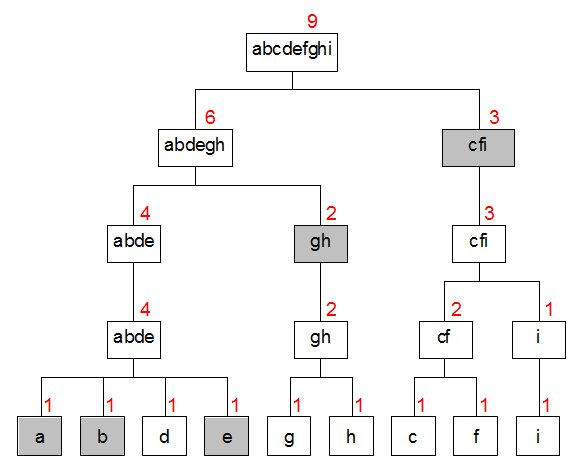
\includegraphics[height=6cm]{ipfs-mnr-addnode1.png}}%
	\hspace{4mm}%
	\subfigure[Add (0,d) itself]{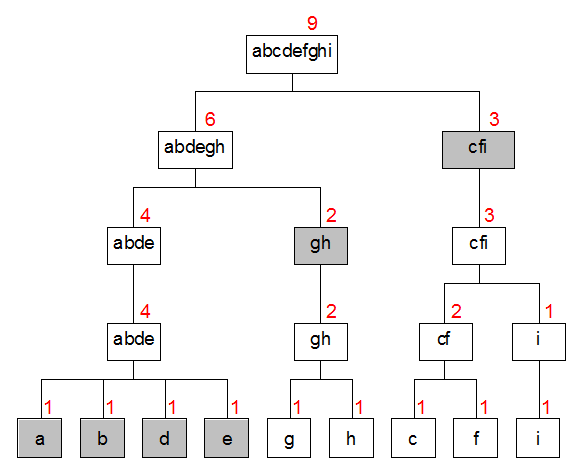
\includegraphics[height=6cm]{ipfs-mnr-addnode2.png}}%
	\hspace{4mm}%
	\subfigure[Consolidate (1,abde)]{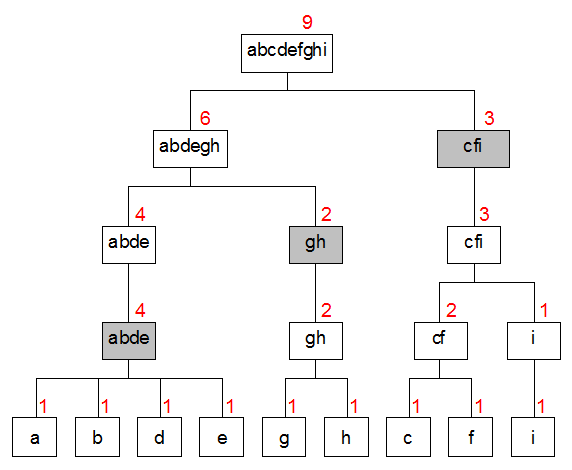
\includegraphics[height=6cm]{ipfs-mnr-addnode3.png}}%
	\hspace{4mm}%
	\subfigure[Consolidate (2,abde)]{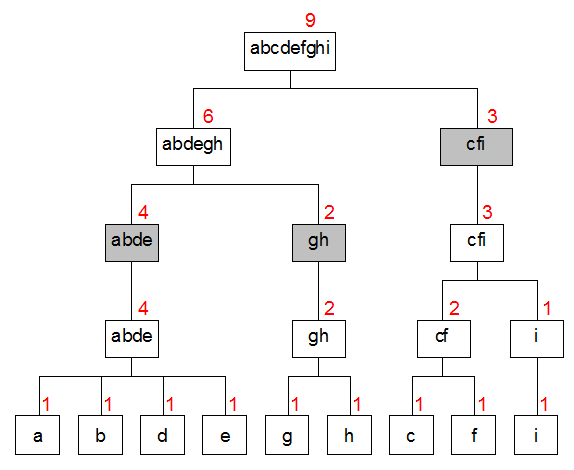
\includegraphics[height=6cm]{ipfs-mnr-addnode4.png}}%
	\hspace{4mm}%
	\subfigure[Consolidate (3,abdegh)]{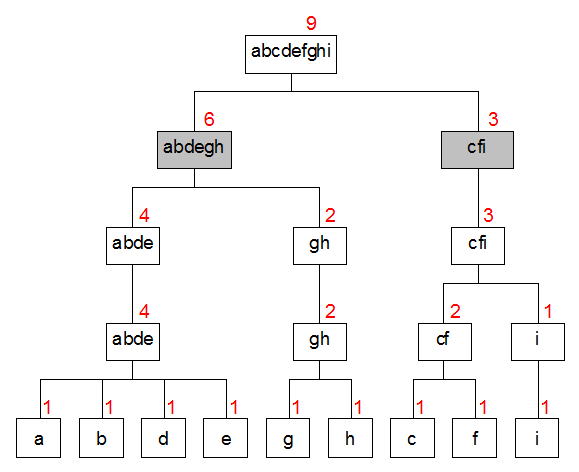
\includegraphics[height=6cm]{ipfs-mnr-addnode5.png}}%
	\hspace{4mm}%
	\subfigure[Consolidate (4,abcdefghi)]{\includegraphics[height=6cm]{ipfs-mnr-addnode6.png}}%
\end{center}
\caption{Add to Selection Example: Adding (0,d) to an existing selection}
\label{fig:ipfs-mnr-addnode}
\end{figure}
%---

\subsubsection{Remove from Selection}

There are four cases to deal with when removing a node from the selection as well:

\begin{enumerate}

\item The node is in \acronym{MNR}(S) $\Rightarrow$ remove it.
\item An ancestor of the node is in \acronym{MNR}(S); this case will be covered below.
\item Some descendants of the node are in \acronym{MNR}(S) $\Rightarrow$ remove them.
\item Otherwise no part of S lies within the region represented by the node, so do nothing.

\end{enumerate}

The interesting case involves removing a node whose ancestor is in \acronym{MNR}(S). To do this, we find the \emph{trail} of nodes in the tree leading from the ancestor to the node itself. We then recursively split the nodes along this trail until we get back to the original node: the intermediate \acronym{MNR}(S) then contains the original node and we can simply remove it. For example, consider Figure~\ref{fig:ipfs-mnr-addnode} in reverse (i.e.~consider removing $(0,d)$ from the selection in (f)). Here, the trail of nodes from the ancestor (namely $(4,\mathit{abcdefghi})$) is $(4,\mathit{abcdefghi})$, $(3,\mathit{abdegh})$, $(2,\mathit{abde})$, $(1,\mathit{abde})$. Each of these should be split in turn until the representation contains the grey nodes in (b): at this point, removing $(0,d)$ is trivial.

\subsubsection{View at Layer}

The view of a selection at layer $\ell$ is defined to be the selected regions in layers $\le \ell$, plus the descendants at layer $\ell$ of selected regions in layers $> \ell$. This allows large regions in higher layers of the hierarchy to be selected and then viewed in terms of their constituent sub-regions. The view at layer algorithm is thus as follows:

%~
\begin{enumerate}

\item Let $\mathit{ns}$ hold the set of nodes in the view of the selection, initially empty.
\item For each node $n$ in the minimal node representation of the selection:

%~~
\begin{enumerate}
\item If $n$ is in a layer $\le \ell$, add it to $\mathit{ns}$.
\item Otherwise, recursively find the descendants of $n$ in layer $\ell$ and add those to $\mathit{ns}$ instead.
\end{enumerate}
%~~

\end{enumerate}
%~

An example is shown in Figure~\ref{fig:ipfs-mnr-viewatlayer}.

%---
\begin{figure}[p]
\begin{center}
	\subfigure[The MNR of the selection]{\includegraphics[height=6cm]{ipfs-mnr-viewatlayer1.png}}%
	\hspace{4mm}%
	\subfigure[The view at layer 2]{\includegraphics[height=6cm]{ipfs-mnr-viewatlayer2.png}}%
\end{center}
\caption{View at Layer Example}
\label{fig:ipfs-mnr-viewatlayer}
\end{figure}
%---
